$subject$=Физические основы компьютерных \\ и сетевых технологий
$teacher$=Лекции Музыченко Я. Б.
$date$=09.12.2024

\section{13. Электрическое поле в диэлектриках и проводниках. Конденсаторы}

\subsection{Поляризованность}

$\vec{P} = \frac{\sum_{\Delta V} \vec{p}}{\Delta V}$ \hfill $[P] = \frac{\text{Кл}}{\text{м}^2}$

$\vec{P} = \chi \varepsilon_0 \vec{E}$

$\chi \geq 0$ - диэлектрическая восприимчивость ($\chi = 0$ для воздуха и вакуума)

$\vec{P} \uparrow\uparrow \vec{E}$

\begin{minipage}{\textwidth}
    \begin{wrapfigure}{r}{0pt}
        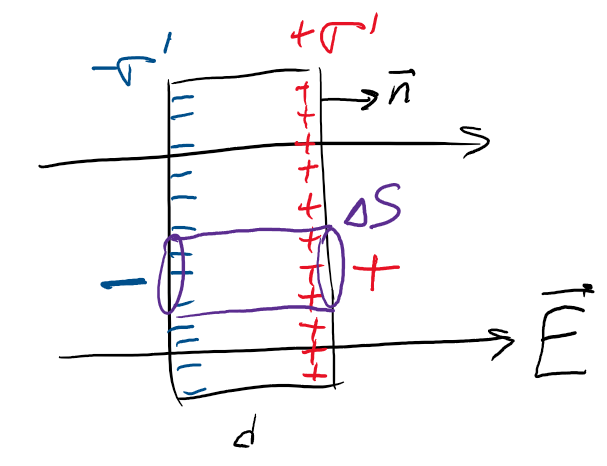
\includegraphics[width=6cm]{physics1/images/physics1_2024_12_09_1}
    \end{wrapfigure}

    Обычно, зависимость поляризованности от напряженности внешнего электрического поля линейна. 
    Однако у сегнетоэлектриков она не линейная - при колебаниях направления напряженности поля зависимость поляризованности
    образует на графике петлю гистерезиса из-за того, что сегнетоэлектрики меняют свою диэлектрическую проницаемость

    Возьмем пластину толщиной $d$. Поместим ее в однородное горизонтальное электрическое поле. 
    По воздействием поля слева на пластине образуется отрицательный заряд, а справа положительный

    Выделем элементарный цилиндр высотой $d$. Его можем представить как диполь

    $|\vec{P}| = \frac{|\sum \vec{p}|}{\Delta V} = \frac{|\vec{p}|}{\Delta V} = \frac{q^\prime d}{\Delta S d} = \frac{q^\prime}{\Delta S} = \sigma^\prime$ - поверхностное распределение заряда

    Для произвольного направления внешнего поля: $P_n = P \cos\alpha = \sigma^\prime$, где $\alpha$ - угол между вектором поляризованности и нормальный вектором к боковой поверхности пластины

\end{minipage}

\subsection{Теорема Гаусса для вектора поляризованности}

\Mems Теорема Гаусса - $\oint \vec{E} d\vec{s} = \frac{q_\text{общ}}{\varepsilon_0}$

Найдем поток $\vec{P}$ через $ds$

$\int \vec{P} d\vec{s} = \int P\cos\alpha ds = \int \sigma^\prime ds = \int dq^\prime = q^\prime$

Если поверхность замкнутая: $\oint \vec{P} d\vec{s} = -q^\prime$ - теорема Гаусса для вектора поляризованности

\subsection{Взаимосвязи $q^\prime$ и $q$ ($\sigma^\prime$ и $\sigma$)}

$\oint \vec{P} d\vec{s} = -q^\prime$

$\vec{P} = \chi \varepsilon_0 \vec{E}$

$\chi \varepsilon_0 \oint \vec{E} d\vec{s} = -q^\prime$

$\chi q_{\text{общ}} = -q^\prime$, где $q_\text{общ} = q_{\text{связ}} + q_\text{своб}$

$\chi (q + q^\prime) = -q^\prime$

$q^\prime = -\frac{\chi q}{1 + \chi}$ - связанный заряд появится только тогда, когда есть свободные

Значит внутри диэлектриков связанных зарядов нет

\subsection{Электрическое смещение (электрическая индукция)}

\Mem $\oint \vec{E} d\vec{s} = \frac{q + q^\prime}{\varepsilon_0}$

$\oint \varepsilon_0 \vec{E} d\vec{s} + \oint \vec{P}d\vec{s} = q$

$\oint (\underset{\vec{D}}{\underbrace{\varepsilon_0 \vec{E} + \vec{P}}}) d\vec{s} = q$

$\vec{D} = \varepsilon_0 \vec{E} + \vec{P}$ - электрическое смещение \hfill $[D] = \frac{\text{Кл}}{\text{м}^2}$

$\vec{D} = \varepsilon_0 \vec{E} + \chi \varepsilon_0 \vec{E} = (1 + \chi) \varepsilon_0 \vec{E} = \varepsilon \varepsilon_0 \vec{E}$

$\varepsilon = 1 + \chi$ - диэлектрическая проницаемость среды

\subsection{Граничные условия}

Возьмем элементарный цилиндр и поместим его на границе двух сред с разными проницаемостями

Тогда при уменьшении высоты цилиндра получим поток через него:

$\Phi = P_{2n} \Delta S - P_{1n} \Delta S = -\sigma^\prime \Delta S$

$P_{2n} - P_{1n} = -\sigma^\prime$

Если какая-то среда не является диэлектриком (например, первая становится воздухом), то $P_{2n} = -\sigma^\prime$

$\xi\varepsilon_0 E_n = -\sigma^\prime$, где $E_n$ - поле внутри диэлектрика

Для электрического смещения:

$\Phi = D_{2n} \Delta S - D_{1n} \Delta S = q_\text{своб}$

$D_{2n} - D_{1n} = \sigma_\text{своб}$ 

Но для диэлектриков $q_\text{своб} = 0$, поэтому $D_{2n} = D_{1n}$

Для напряженности:

$\oint \vec{E} d\vec{l} = E_{\tau 2} l \cdot E_{\tau 1} l = 0$ по теореме о циркуляции

$E_{\tau 2} = E_{\tau 1}$

Линии напряженности поля преломляются на границе двух сред

\begin{center}
    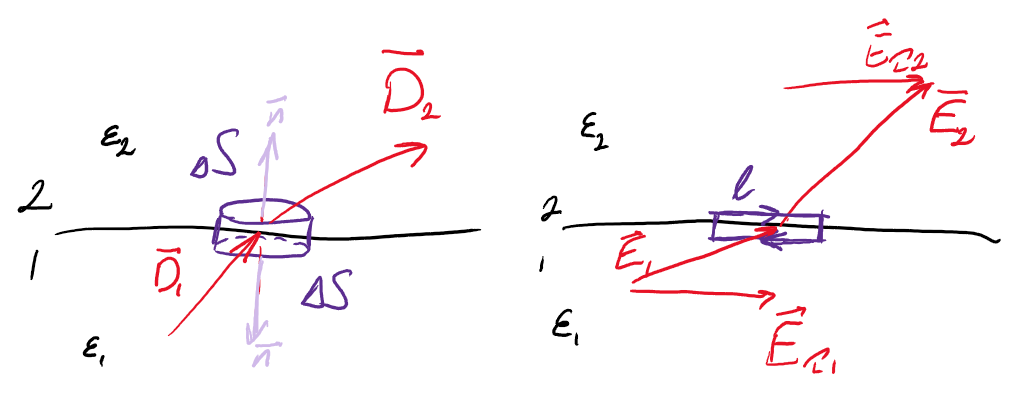
\includegraphics[width=0.8\textwidth]{physics1/images/physics1_2024_12_09_2}
\end{center}

\subsection{Конденсатор}

Конденсатор - две пластины, между которыми есть разность потенциалов. Из-за этого конденсатор может иметь электроемкость, которую измеряют в фарадах

$C = \frac{q}{\varphi}$ \hfill $[C] = \text{Ф}$

Для плоского конденсатора:

$C = \frac{q}{U} = \frac{q}{Ed} = \frac{q \varepsilon_0 \varepsilon}{d\sigma} = \frac{\varepsilon \varepsilon_0 S}{d}$

Для цилиндрического конденсатора:

$C = \frac{q}{U} = \frac{q}{\int \vec{E}d\vec{l}} = \frac{l \cdot 2\pi \varepsilon \varepsilon_0}{\ln \frac{r_2}{r_1}}$


